\documentclass[journal,12pt,twocolumn]{IEEEtran}
%
\usepackage{setspace}
\usepackage{gensymb}
%\doublespacing
\singlespacing

%\usepackage{graphicx}
%\usepackage{amssymb}
%\usepackage{relsize}
\usepackage[cmex10]{amsmath}
%\usepackage{amsthm}
%\interdisplaylinepenalty=2500
%\savesymbol{iint}
%\usepackage{txfonts}
%\restoresymbol{TXF}{iint}
%\usepackage{wasysym}
\usepackage{amsthm}
%\usepackage{iithtlc}
\usepackage{mathrsfs}
\usepackage{txfonts}
\usepackage{stfloats}
\usepackage{bm}
\usepackage{cite}
\usepackage{cases}
\usepackage{subfig}
%\usepackage{xtab}
\usepackage{longtable}
\usepackage{multirow}
%\usepackage{algorithm}
%\usepackage{algpseudocode}
\usepackage{enumitem}
\usepackage{mathtools}
\usepackage{steinmetz}
\usepackage{tikz}
\usepackage{circuitikz}
\usepackage{verbatim}
\usepackage{tfrupee}
\usepackage[breaklinks=true]{hyperref}
%\usepackage{stmaryrd}
\usepackage{tkz-euclide} % loads  TikZ and tkz-base
%\usetkzobj{all}
\usetikzlibrary{calc,math}
\usepackage{listings}
    \usepackage{color}                                            %%
    \usepackage{array}                                            %%
    \usepackage{longtable}                                        %%
    \usepackage{calc}                                             %%
    \usepackage{multirow}                                         %%
    \usepackage{hhline}                                           %%
    \usepackage{ifthen}                                           %%
  %optionally (for landscape tables embedded in another document): %%
    \usepackage{lscape}     
\usepackage{multicol}
\usepackage{chngcntr}
%\usepackage{enumerate}

%\usepackage{wasysym}
%\newcounter{MYtempeqncnt}
\DeclareMathOperator*{\Res}{Res}
%\renewcommand{\baselinestretch}{2}
\renewcommand\thesection{\arabic{section}}
\renewcommand\thesubsection{\thesection.\arabic{subsection}}
\renewcommand\thesubsubsection{\thesubsection.\arabic{subsubsection}}

\renewcommand\thesectiondis{\arabic{section}}
\renewcommand\thesubsectiondis{\thesectiondis.\arabic{subsection}}
\renewcommand\thesubsubsectiondis{\thesubsectiondis.\arabic{subsubsection}}

% correct bad hyphenation here
\hyphenation{op-tical net-works semi-conduc-tor}
\def\inputGnumericTable{}                                 %%

\lstset{
%language=C,
frame=single, 
breaklines=true,
columns=fullflexible
}
%\lstset{
%language=tex,
%frame=single, 
%breaklines=true
%}

\begin{document}
%


\newtheorem{theorem}{Theorem}[section]
\newtheorem{problem}{Problem}
\newtheorem{proposition}{Proposition}[section]
\newtheorem{lemma}{Lemma}[section]
\newtheorem{corollary}[theorem]{Corollary}
\newtheorem{example}{Example}[section]
\newtheorem{definition}[problem]{Definition}
%\newtheorem{thm}{Theorem}[section] 
%\newtheorem{defn}[thm]{Definition}
%\newtheorem{algorithm}{Algorithm}[section]
%\newtheorem{cor}{Corollary}
\newcommand{\BEQA}{\begin{eqnarray}}
\newcommand{\EEQA}{\end{eqnarray}}
\newcommand{\define}{\stackrel{\triangle}{=}}

\bibliographystyle{IEEEtran}
%\bibliographystyle{ieeetr}


\providecommand{\mbf}{\mathbf}
\providecommand{\pr}[1]{\ensuremath{\Pr\left(#1\right)}}
\providecommand{\qfunc}[1]{\ensuremath{Q\left(#1\right)}}
\providecommand{\sbrak}[1]{\ensuremath{{}\left[#1\right]}}
\providecommand{\lsbrak}[1]{\ensuremath{{}\left[#1\right.}}
\providecommand{\rsbrak}[1]{\ensuremath{{}\left.#1\right]}}
\providecommand{\brak}[1]{\ensuremath{\left(#1\right)}}
\providecommand{\lbrak}[1]{\ensuremath{\left(#1\right.}}
\providecommand{\rbrak}[1]{\ensuremath{\left.#1\right)}}
\providecommand{\cbrak}[1]{\ensuremath{\left\{#1\right\}}}
\providecommand{\lcbrak}[1]{\ensuremath{\left\{#1\right.}}
\providecommand{\rcbrak}[1]{\ensuremath{\left.#1\right\}}}
\theoremstyle{remark}
\newtheorem{rem}{Remark}
\newcommand{\sgn}{\mathop{\mathrm{sgn}}}
\providecommand{\abs}[1]{\left\vert#1\right\vert}
\providecommand{\res}[1]{\Res\displaylimits_{#1}} 
\providecommand{\norm}[1]{\left\lVert#1\right\rVert}
%\providecommand{\norm}[1]{\lVert#1\rVert}
\providecommand{\mtx}[1]{\mathbf{#1}}
\providecommand{\mean}[1]{E\left[ #1 \right]}
\providecommand{\fourier}{\overset{\mathcal{F}}{ \rightleftharpoons}}
%\providecommand{\hilbert}{\overset{\mathcal{H}}{ \rightleftharpoons}}
\providecommand{\system}{\overset{\mathcal{H}}{ \longleftrightarrow}}
	%\newcommand{\solution}[2]{\textbf{Solution:}{#1}}
\newcommand{\solution}{\noindent \textbf{Solution: }}
\newcommand{\cosec}{\,\text{cosec}\,}
\providecommand{\dec}[2]{\ensuremath{\overset{#1}{\underset{#2}{\gtrless}}}}
\newcommand{\myvec}[1]{\ensuremath{\begin{pmatrix}#1\end{pmatrix}}}
\newcommand{\mydet}[1]{\ensuremath{\begin{vmatrix}#1\end{vmatrix}}}
%\numberwithin{equation}{section}
\numberwithin{equation}{subsection}
%\numberwithin{problem}{section}
%\numberwithin{definition}{section}
\makeatletter
\@addtoreset{figure}{problem}
\makeatother

\let\StandardTheFigure\thefigure
\let\vec\mathbf
%\renewcommand{\thefigure}{\theproblem.\arabic{figure}}
\renewcommand{\thefigure}{\theproblem}
%\setlist[enumerate,1]{before=\renewcommand\theequation{\theenumi.\arabic{equation}}
%\counterwithin{equation}{enumi}


%\renewcommand{\theequation}{\arabic{subsection}.\arabic{equation}}

\def\putbox#1#2#3{\makebox[0in][l]{\makebox[#1][l]{}\raisebox{\baselineskip}[0in][0in]{\raisebox{#2}[0in][0in]{#3}}}}
     \def\rightbox#1{\makebox[0in][r]{#1}}
     \def\centbox#1{\makebox[0in]{#1}}
     \def\topbox#1{\raisebox{-\baselineskip}[0in][0in]{#1}}
     \def\midbox#1{\raisebox{-0.5\baselineskip}[0in][0in]{#1}}

\vspace{3cm}


\title{Que: 11.10.3.17}
\author{Nikam Pratik Balasaheb (EE21BTECH11037)}





% make the title area
\maketitle

\newpage

%\tableofcontents

\bigskip

\renewcommand{\thefigure}{\theenumi}
\renewcommand{\thetable}{\theenumi}
%\renewcommand{\theequation}{\theenumi}

\section{Problem}

In triangle ABC with vertices $\vec{A} = \myvec{2\\3}$, $\vec{B} = \myvec{4\\-1}$ and $\vec{C}= \myvec{1\\2}$, FInd the equation and length of altitude from vertex $\vec{A}$
\section{Solution}

\begin{enumerate}

\item Direction vector of side BC
	\begin{align}
		\vec{m} &= \vec{B} - \vec{C} \\
		&= \myvec{3 \\ -3} 
	\end{align}

 Direction vector of side BC is normal of altitude from $\vec{A}$

\item Equation of the altitude
	\begin{align}
		\vec{m}^{\top} \brak{\vec{x} - \vec{A}} &= 0 \\
		\myvec{3 & -3} \vec{x} &=  -3 \\
		\myvec{1 & -1} \vec{x} &=  -1
	\end{align}

\item Equation of line BC
	\begin{align}
		\vec{x} &= \vec{B} + \mu \vec{m}  \\
		\vec{x} &= \myvec{4 \\ -1} + \mu \myvec{3 \\ -3} \\
		i.e. \; \; \myvec{1 & 1} \vec{x} &=  3
	\end{align}

\item Optimization problem

	The length of altitude can be expressed as a optimization problem,
		\begin{align}
			\text{min} \norm{\vec{A} - \vec{x}}^2  \label{eq:1}
		\end{align}

		such that 
		\begin{align}
			\vec{n}^{\top} \vec{x} &=  c
		\end{align}

		where,
		\begin{align}
			\vec{n} &= \myvec{1\\1} \\
			c &= 3
		\end{align}

		\eqref{eq:1} is solved using Gradient Descent in \texttt{codes/11.10.3.17.py}. 
		The results obtained are using 0.01 as learning rate, iterated until the diffrence between cost in consecutive iterations is lesser than $5 \times 10^{-7}$.
		\\
		The results obtained are:

		\begin{align}
			\mu_{min} & = -0.99986708\\
			\text{min}\norm{\vec{A} - \vec{x}}^2 & = 2.000000318
		\end{align}

Therefore, the length of altitude is given by,
		\begin{align}
			l &= \sqrt{2} \approx 1.414213562
		\end{align}

\begin{comment}
	\item	The line equation can be expressed as
		\begin{align}
			\vec{x} &= \vec{B} + \mu \vec{m}
		\end{align}
	where,
		\begin{align}
			\vec{m} &= \myvec{3\\-3} \\
			\vec{B} &= \myvec{4\\-1}
		\end{align}

	Substituting in the optimization problem,

	\begin{align}
		\text{min} \norm{\vec{A} - \brak{\vec{B} + \mu \vec{m}} }^2\\
		\text{min} \; f(\mu) = \mu^2 \norm{\vec{m}}^2 - 2 \mu \vec{m}^{\top} \brak{\vec{A} - \vec{B}} + \norm{\vec{A} - \vec{B}}^2
	\end{align}
		
	 coefficient of $\mu^2$ is positive, the function is convex.

	\begin{align}
		f''(\mu) &= 2 \norm{\vec{m}}^2 > 0\\
		\therefore f'(\mu_{min}) &= 0
	\end{align}

	\begin{align}
                \frac{\partial f}{\partial \mu} &= - 2 \vec{m}^{\top} \brak{\vec{A} - \vec{B}} + 2 \mu \norm{\vec{m}}^2 = 0 \\
		\mu_{min} &= \frac{\vec{m}^{\top} \brak{\vec{A} - \vec{B}}}{\norm{\vec{m}}^2} \\
                &= \frac{\myvec{3 & -3} \myvec{-2 \\ 4}}{18} \\
                &= \frac{-18}{18} \\
                &= -1
        \end{align}
	
	Substituting in the line equation,

	\begin{align}
		\vec{x}_{min} &= \vec{B} + \mu_{min} \vec{m} \\ 
		&= \myvec{1\\2}
	\end{align}


\item 	Length of altitude,

	\begin{align}
		l &= \norm{\vec{A} - \vec{x}_{min}} \\
		&= \sqrt{2}
	\end{align}

\end{comment}

\end{enumerate}

\begin{table}[h!] 
\centering
        %%%%%%%%%%%%%%%%%%%%%%%%%%%%%%%%%%%%%%%%%%%%%%%%%%%%%%%%%%%%%%%%%%%%%%
%%                                                                  %%
%%  This is a LaTeX2e table fragment exported from Gnumeric.        %%
%%                                                                  %%
%%%%%%%%%%%%%%%%%%%%%%%%%%%%%%%%%%%%%%%%%%%%%%%%%%%%%%%%%%%%%%%%%%%%%%

\begin{tabular}[]{|c|c|c|}
\hline
Parameter	& Value		& Description\\ \hline
$\vec{O}$	& $\myvec{5\\0}$ &Center of the given circle \\ \hline
$\vec{B}$	& $\myvec{0\\0}$ &Point where Salma is standing\\ \hline
$r$		& 5 & radius of given circle \\ \hline
$d$ 		& 6 & distance AB and BC\\ \hline
\end{tabular}

        \caption{Table}
        \label{tab:}
\end{table} 

\begin{figure}[h!]
  \centering
   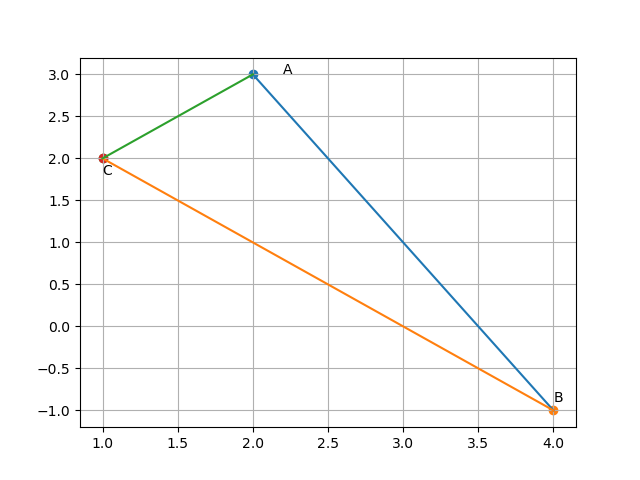
\includegraphics[width=\linewidth]{figs/figure_1.png}
   \caption{Figure}
   \label{fig:}
\end{figure}

%Note that $\vec{x}_{min}$ i.e. the foot of the altitude is co-incident with the vertex $\vec{C}$. Therefore, the altitude is side AC itself.



\end{document}

